\documentclass{article}
\usepackage[utf8]{inputenc}
\usepackage[spanish]{babel}
\usepackage{amsmath}
\usepackage{amssymb}
\usepackage{amsfonts}
\usepackage{hyperref}
\usepackage{textcomp}
\usepackage{graphicx}
\usepackage{pgfplots}
\usepackage{geometry}
\hypersetup{
    colorlinks=true,
    linkcolor=black,
    citecolor=green,
    filecolor=magenta,      
    urlcolor=cyan,
}
\geometry{
  top=3cm,            % Margen superior
  bottom=3cm,         % Margen inferior
  left=3cm,           % Margen izquierdo
  right=3cm           % Margen derecho
}

\title{Estadística 1}
\author{Jorge Miguel Alvarado Reyes}
\date{16 Agosto 2023}

\setlength{\parindent}{0pt}
\begin{document}

\begin{titlepage}
    \begin{center}
        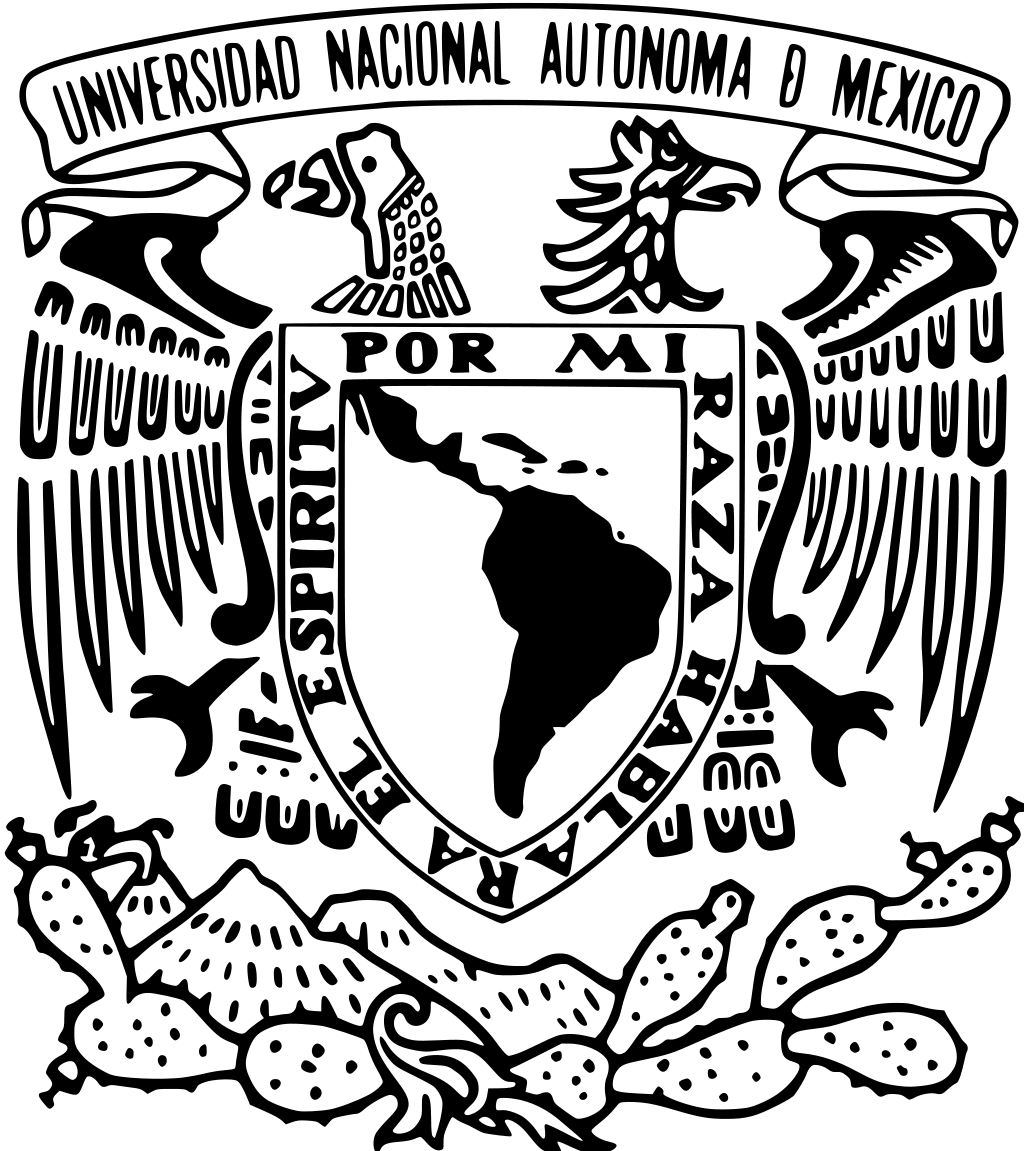
\includegraphics[width=0.2\textwidth]{../../unam.png}
        \vspace*{.5cm}

        \LARGE
        \textbf{Universidad Nacional Autónoma de México}

        \vspace{0.5cm}
        \LARGE
        Facultad de Estudios Superiores Acatlán

        \vspace{2cm}

        \textbf{Examen Unidad 1} \\
        Ecuaciones Diferenciales

        \vfill

        \vspace{1cm}

        \textbf{\large Autor:} \\
        Jorge Miguel Alvarado Reyes \\
        421010301\\
        \vspace{.5cm}
        \normalsize \today

    \end{center}
\end{titlepage}
\newpage

\tableofcontents

\newpage
\section{1}
Observe que $\mathcal{L} \left\{ \int_{0}^{t} f(\tau) d\tau \right\} =  \frac{F(s)}{s} $,  Determine la transformada de Laplace de las siguientes funciones


\subsection*{1.1}

\[f(\tau) = \cos(\tau - a)\]

\subsection*{Solucion}

\[ \int_{0}^{t} \cos(\tau - a) d\tau \]

Usando la sustitución

\[u = \tau - a, \hspace*{.5cm}, du = d\tau\]

Cambiando los limites de integracion

\begin{align*}
    \int_{-a}^{t-a} \cos(u) \, du & = \sen(u) \Bigg|_{-a}^{t-a} \\
                                  & = \sen(t-a) - \sen(-a)      \\
                                  & = \sen(t-a) + \sen(a)       \\
\end{align*}

\[
    \mathcal{L}\{\sen(t-a) + \sen(a)\} = \mathcal{L}\{\sen(t-a)\} + \mathcal{L}\{\sen(a)\}
\]

Calulando $\mathcal{L}\{\sen(t-a)\}$

\[
    \mathcal{L}\{\sen(t-a)\} = \mathcal{L}\{sin(t)cos(a) - cos(t)sen(a)\}
\]

\[
    \begin{aligned}
        \mathcal{L}\{\sen t \cos a - \cos t \sen a\} & = \cos a \cdot \mathcal{L}\{\sen t\} - \sen a \cdot \mathcal{L}\{\cos t\} \\
                                                     & = \cos a \cdot \frac{1}{s^2 + 1} - \sen a \cdot \frac{s}{s^2 + 1}         \\
                                                     & = \frac{\cos a - s \sen a}{s^2 + 1}
    \end{aligned}
\]

\[
    \mathcal{L}\{\sen(t-a) + \sen(a)\} = \frac{\cos a - s \sen a}{s^2 + 1} + \frac{sen(a)}{s} = \frac{scos(a) + sen(a)}{s^3+s}
\]

\begin{center}
    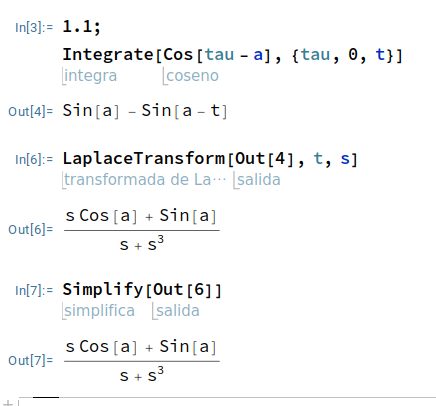
\includegraphics[width=0.5\textwidth]{./image5.png}
\end{center}

\subsection*{1.4}

\[f(\tau) = 2\tau\sen(\tau+a)\]

\subsection*{Solucion}

\[ \int_{0}^{t} 2\tau \sen(\tau+a) \, d\tau \]

\[ \sen(\tau+a) = \sen\tau\cos a + \cos\tau\sen a \]

Ahora reemplazamos esta expresión en la integral:

\[ \int_{0}^{t} 2\tau (\sen\tau\cos a + \cos\tau\sen a) \, d\tau \]

Separamos la integral:

\[ \int_{0}^{t} 2\tau\sen\tau\cos a \, d\tau + \int_{0}^{t} 2\tau\cos\tau\sen a \, d\tau \]

Resolviendo la primera parte:

1. \[ \int_{0}^{t} 2\tau\sen\tau\cos a \, d\tau = 2cos(a)(-tcos(t) + sen(t))\]

\begin{center}
    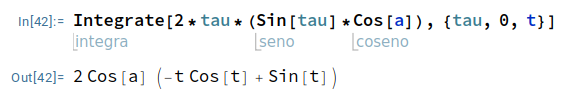
\includegraphics[width=0.5\textwidth]{./image6.png}
\end{center}

Ahora resolvamos la segunda integral:

2. \[ \int_{0}^{t} 2\tau\cos\tau\sen a \, d\tau = 2sen(a)(-1+cos(t) + tsen(t))\]

\begin{center}
    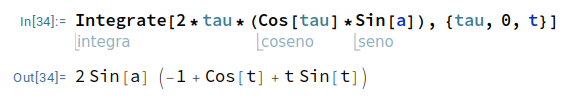
\includegraphics[width=0.5\textwidth]{./image7.png}
\end{center}

Ahora juntando ambas integrales obtenidas:

\[ \int_{0}^{t} 2\tau \sen(\tau+a) \, d\tau = 2cos(a)(-tcos(t) + sen(t)) +  2sen(a)(-1+cos(t) + tsen(t))\]

\[ \int_{0}^{t} 2\tau \sen(\tau+a) \, d\tau = -2(t cos(a+t) + sen(a) -sen(a+t))\]

Ahora calculamos la tranformada de laplace de la integral

\[
    \mathcal{L}\{-2(t cos(a+t) + sen(a) -sen(a+t))\}
\]
\begin{center}
    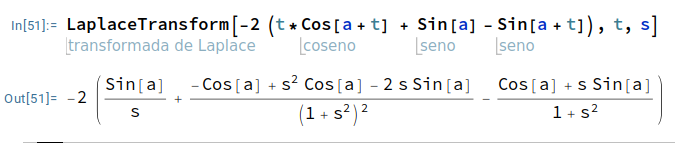
\includegraphics[width=0.5\textwidth]{./image8.png}
\end{center}

\newpage
\section{2}
Demuestre que la Transformada de Laplace de una convolución de dos funciones es

\[
    \mathcal{L} \{ f*g \} = F(s)G(s) \quad \text{donde} \quad f*g = \int_{0}^{t} f(\tau) g(t - \tau) d\tau
\]

\begin{center}
    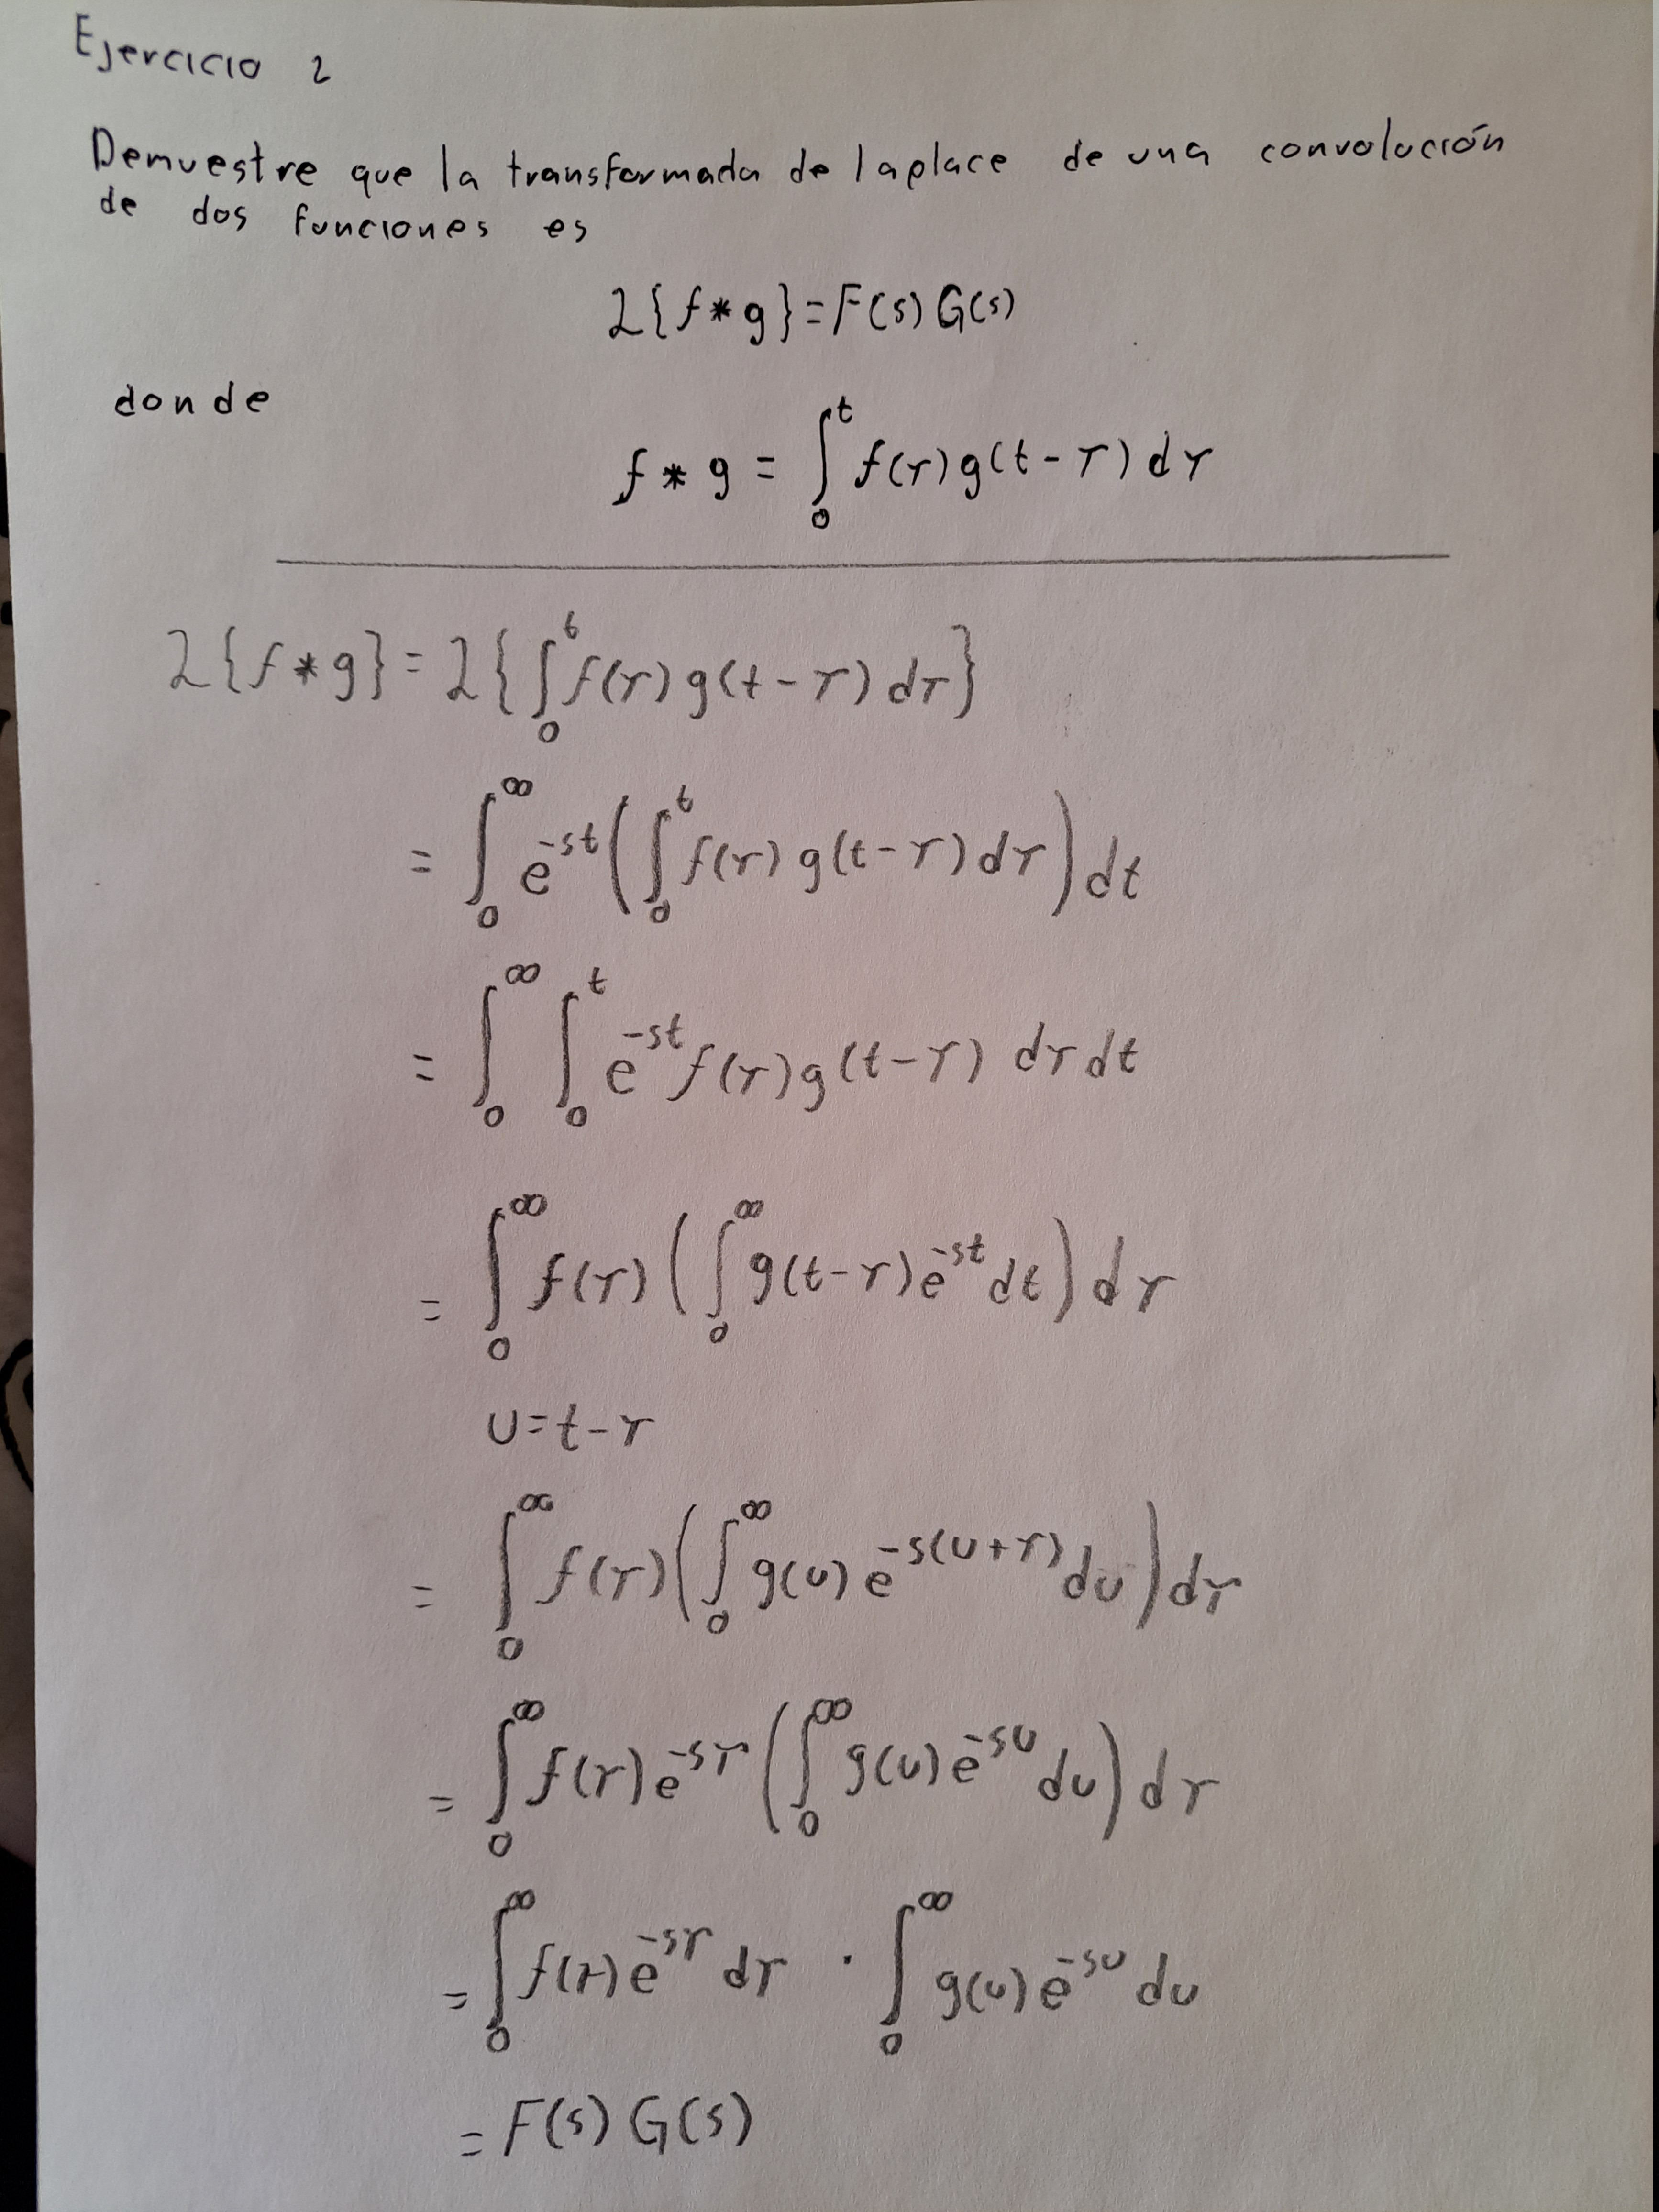
\includegraphics[width=\textwidth]{./ejercicio2.jpg}
\end{center}

\section{3}
Observe entonces que

\[
    \mathcal{L}^{-1}\{F(s)G(s)\} = \int_0^{\infty} f(\tau)g(t - \tau) \, d\tau,
\]
Determine la Transformada Inversa de Laplace de

\subsection{3.1}
\[
    F(s) = \frac{7}{s^4}, \quad G(s) = \frac{2}{(s^2-4s+13)}
\]
\subsection*{Solucion}

Calculando $\mathcal{L}^{-1}\left\{F(s)\right\} $

\[
    \mathcal{L}^{-1}\left\{\frac{7}{s^4}\right\} = \frac{t^{4-1}}{(4-1)!} = \frac{7t^3}{6}
\]

Calculando $\mathcal{L}^{-1}\left\{G(s)\right\} $

\[
    \mathcal{L}^{-1}\left\{\frac{2}{(s^2-4s+13)}\right\} = 2\mathcal{L}^{-1}\left\{\frac{1}{(s-2)^2+3^2}\right\}
\]

Usando

\[
    \mathcal{L}^{-1}\left\{ \frac{1}{(s - a)^2 + b^2} \right\} = e^{at} \sen(bt)
\]

\[
    2\mathcal{L}^{-1}\left\{\frac{1}{(s-2)^2+3^2}\right\} =  2 e^{2t} \cos(3t)
\]

Por lo tanto nuestras $f(t)$ y $g(t)$ son

\[
    f(t) = \frac{7t^3}{6}, \quad g(t) =2 e^{2t} \cos(3t)
\]

Por lo tanto la convolucion es:

\[
    f(t) \ast g(t) = \int_{0}^{t} f(\tau) \cdot g(t - \tau) \, d\tau
\]

Sustituyendo las funciones:

\[
    f(t) \ast g(t) = \int_{0}^{t} \frac{7\tau^3}{6} \cdot 2 e^{2(t - \tau)} \cos(3(t - \tau)) \, d\tau
\]

\begin{center}
    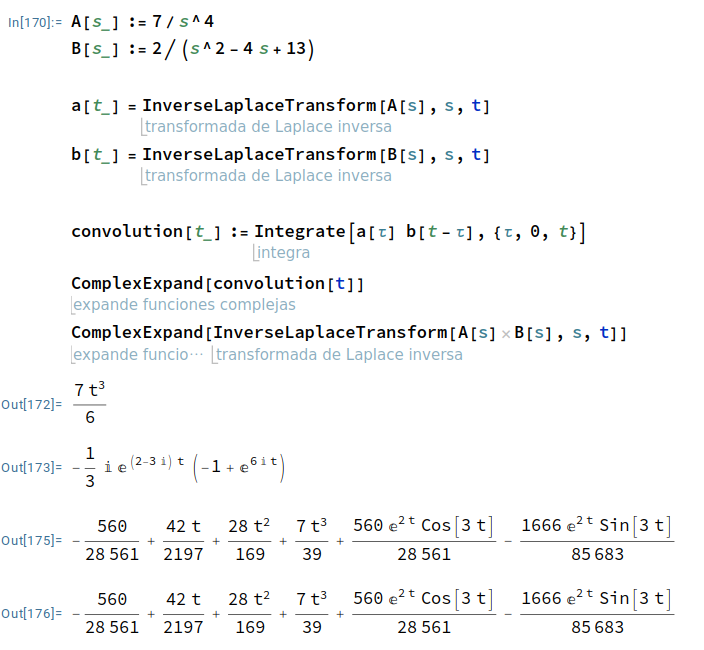
\includegraphics[width=0.7\textwidth]{./image4.png}
\end{center}

\subsection{3.4}
\[
    F(s) = \frac{7s^2+7s-14}{s^6+3s^4+3s^2+1}, \quad G(s) = \frac{2}{s^2}
\]

\subsection*{Solucion}

Dado $G(s) = \frac{2}{s^2}$, podemos aplicar directamente la definición para encontrar la transformada inversa de Laplace:

\[
    \mathcal{L}^{-1}\left\{\frac{2}{s^2}\right\} = \frac{t^{2-1}}{(2-1)!} = 2t = g(t)
\]

Para $F(s) = \frac{7s^2+7s-14}{s^6+3s^4+3s^2+1}$, primero observamos que el denominador puede ser reescrito como $(s^2 + 1)^3$. Entonces, tenemos:

\[
    F(s) = \frac{7s^2 + 7s -14}{(s^2 + 1)^3}
\]

La descomposición en fracciones parciales de $F(s)$ nos da:

\begin{center}
    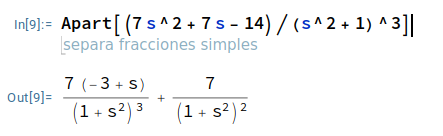
\includegraphics[width=0.6\textwidth]{./image.png}
\end{center}

\[F(s) = \frac{7(s-3)}{(s^2 + 1)^3} + \frac{7}{(s^2 + 1)^2}\]

Para encontrar la transformada inversa de Laplace, aplicamos las reglas correspondientes para cada término:

\begin{center}
    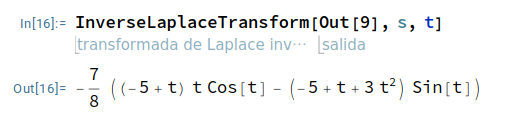
\includegraphics[width=0.6\textwidth]{./image2.png}
\end{center}

\[
    \mathcal{L}^{-1}\left\{\frac{7(s-3)}{(s^2 + 1)^3} + \frac{7}{(s^2 + 1)^2}\right\} = -\frac{7}{8} \left((-5 + t) t\cos(t) - (-5+t+3t^2)\sen(t)\right) = f(t)
\]

El producto de convolución, que es la transformada inversa de Laplace del producto de $F(s)$ y $G(s)$, se define como:

\[
    \mathcal{L}^{-1}\{F(s)G(s)\} = \int_0^{\infty} f(\tau)g(t - \tau) \, d\tau
\]

donde $f(t)$ y $g(t)$ son las transformadas inversas de Laplace de $F(s)$ y $G(s)$ respectivamente. En este caso, necesitaríamos calcular la integral:

\[
    \int_0^{\infty} \left(-\frac{7}{8} \left((-5 + \tau) \tau\cos(\tau) - (-5+\tau+3\tau^2)\sen(\tau)\right)\right)(2(t - \tau)) \, d\tau
\]

Al resover esta integral obtendremos la transformada de laplace

\begin{center}
    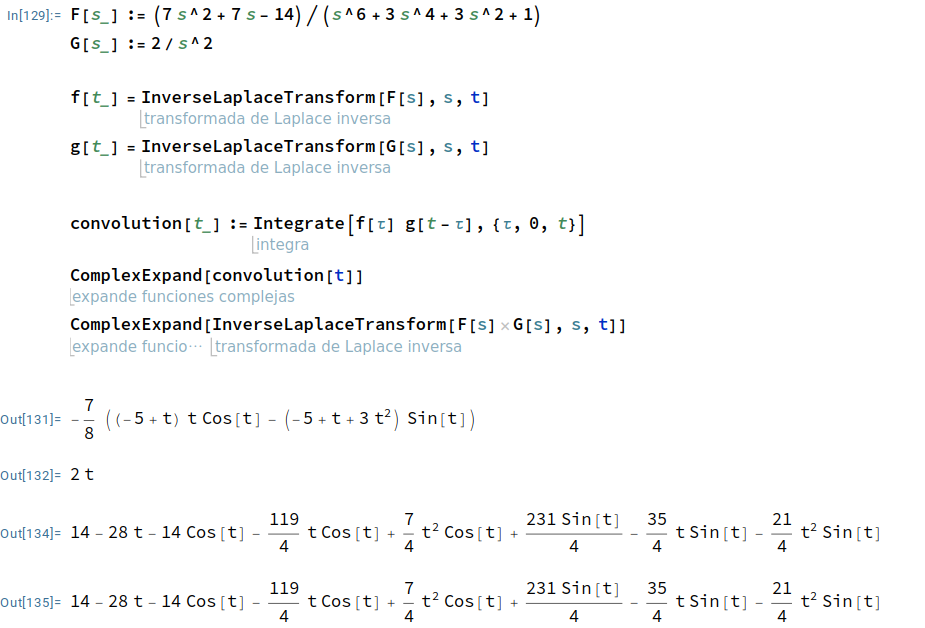
\includegraphics[width=0.7\textwidth]{./image3.png}
\end{center}

En esta caputra podemos confirmar que realizar la inversa de laplace de $F(s)$ y $G(s)$ para obtener $f(t)$ y $g(t)$ y despues calcular su convolucion da el mismo resultado que calcular la inversa de $F(s)$ y $G(s)$

\section{4}
Encuentre la solución de las siguientes ecuaciones diferenciales.

\subsection{4.1}

\[
    y''(t) + 2y'(t) + 2y(t) = \delta(t-5), \quad y(0)=1, \quad y'(0)=0
\]
\subsection{4.2}

\[
    y''(t) + 4y'(t) + 3y(t) = 1 + \delta(t-3), y(0)=0, y'(0) = 1
\]
\end{document}